\begin{minipage}{.35\textwidth}
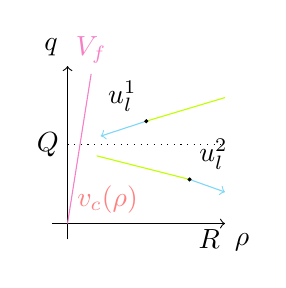
\begin{tikzpicture}
% coordinates
\draw[->] (0,-0.2) -- (0,2) node[anchor= south east] {$q$};
\draw[->] (-0.2,0) -- (2,0) node[anchor= north west] {$\rho$};
% rarefactions
\draw[<-][cyan!50] (0.42, 1.11) -- (1, 1.3) ;
\draw[lime] (1, 1.3) -- (2, 1.6) ;

\draw[->][cyan!50] (1.55,0.56)  -- (2, 0.4) ;
\draw[-][lime] (0.37, 0.86) -- (1.55,0.56)  ;


% v_c
\draw[red!50, domain=0:0.69]  plot[id=x] function{x*(3*x+1)}  node[anchor= south west] {$v_c(\rho)$};
% V_f
\draw[magenta!50] (0,0) -- (0.3, 1.9);
\node[magenta!50] at (0.3, 2.2) {$V_f$};

\draw[dotted] (0,1) -- (2, 1);

\filldraw[black] (1,1.3) circle (0.5pt) node[anchor = south east]{$u_l^1$} ;
\filldraw[black] (1.55,0.56) circle (0.5pt) node[anchor = south west]{$u_l^2$} ;
% contacts
\draw[ orange!50, domain=0:1.86]  plot[id=x] function{(x/1.38)*(2-1.38)/(2-x)*0.33};
\draw[ orange!50, domain=0:1.28]  plot[id=x] function{(x/1.16)*(2-1.16)/(2-x)*1.63};
%
%\node at (1, 1.55) {$u_l$};
\node at (1.8, -0.2) {$R$};
\node at (-0.25, 1) {$Q$};
\end{tikzpicture}
\caption{Wave solutions from two starting points $u_l^1$ and $u_l^2$. }
\label{Fig:FullSol_ic_rhoq}
\end{minipage}
\quad \quad \quad \quad 
\begin{minipage}{.35\textwidth}
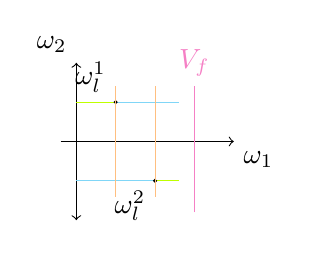
\begin{tikzpicture}
% coordinates
\draw[<->] (0,0) -- (0,2) node[anchor= south east] {$\omega_2$};
\draw[->] (-0.2,1) -- (2,1) node[anchor= north west] {$\omega_1$};
% rarefactions
% rarefactions
\draw[lime] (0, 1.5) -- (0.5, 1.5) ;
\draw[cyan!50] (0.5, 1.5) -- (1.3, 1.5)  ;
\filldraw[black] (0.5, 1.5) circle (0.5pt) node[anchor = south east]{$\omega_l^1$} ;

\draw[cyan!50] (0, 0.5) -- (1, 0.5) ;
\draw[lime] (1, 0.5) -- (1.3, 0.5) ;
\filldraw[black] (1, 0.5)  circle (0.5pt) node[anchor = north east]{$\omega_l^2$} ;

% contacts
\draw[orange!50] (0.5, 1.7) -- (0.5, 0.3) ;
\draw[orange!50] (1, 1.7) -- (1, 0.3) ;

% free ph line
\draw[magenta!50] (1.5, 0.1) -- (1.5, 1.7); 
\node[magenta!50] at (1.5, 2) {$V_f$};
%\filldraw[black] (1.5, 1.5)  circle (0.5pt) node[anchor =  west]{$\omega_r^2$} ;
%\filldraw[black] (1.5, 0.5)  circle (0.5pt) node[anchor = west]{$\omega_r^2$} ;

\end{tikzpicture}
\caption{Wave solutions from two starting points $\omega_l^1$ and $\omega_l^2$.}
\label{Fig:FullSol_ic_ww}
\end{minipage}